\documentclass{standalone}
\usepackage{tikz}
\usetikzlibrary{patterns, positioning}
\usepackage[sfdefault]{ClearSans} %% option 'sfdefault' activates Clear Sans as the default text font
\usepackage[T1]{fontenc}

\begin{document}
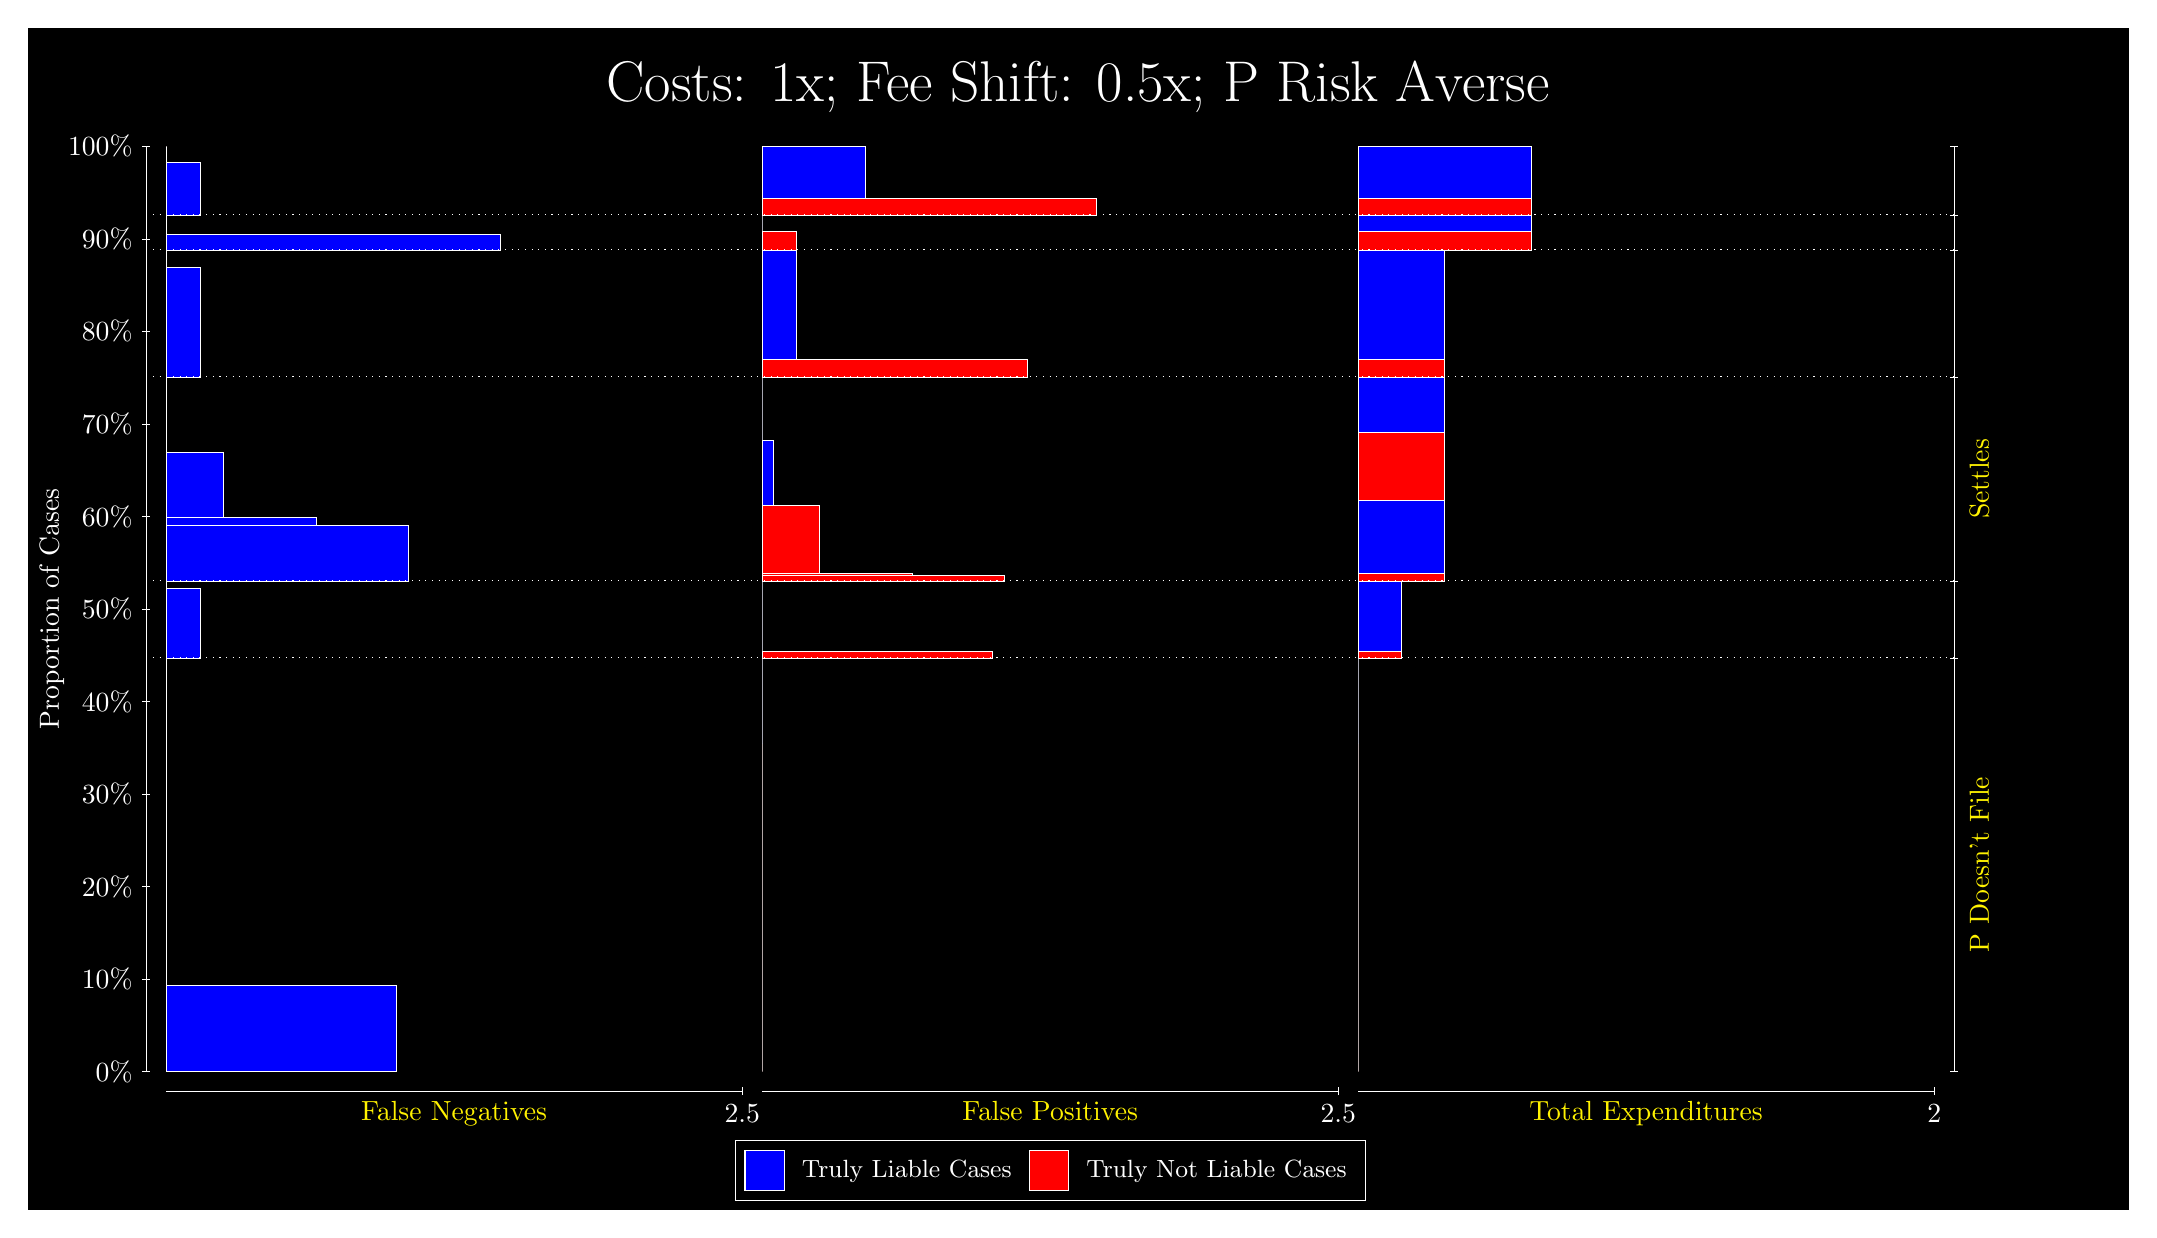
\begin{tikzpicture}
\draw[fill=black] (0,0) rectangle (26.667,15);
\draw[text=white] (0,13.5) rectangle (26.667,15) node[midway] {\huge Costs: 1x; Fee Shift: 0.5x; P Risk Averse};
\draw[white, very thin] (1.5,1.75) -- (1.5,13.5);
\node[rotate=90, text=white, anchor=center] at (0.3, 7.625) {Proportion of Cases};
\draw[white, very thin] (1.45,1.75) -- (1.55,1.75);
\node[text=white, anchor=east] at (1.45, 1.75) {0\%};
\draw[white, very thin] (1.45,2.925) -- (1.55,2.925);
\node[text=white, anchor=east] at (1.45, 2.925) {10\%};
\draw[white, very thin] (1.45,4.1) -- (1.55,4.1);
\node[text=white, anchor=east] at (1.45, 4.1) {20\%};
\draw[white, very thin] (1.45,5.275) -- (1.55,5.275);
\node[text=white, anchor=east] at (1.45, 5.275) {30\%};
\draw[white, very thin] (1.45,6.45) -- (1.55,6.45);
\node[text=white, anchor=east] at (1.45, 6.45) {40\%};
\draw[white, very thin] (1.45,7.625) -- (1.55,7.625);
\node[text=white, anchor=east] at (1.45, 7.625) {50\%};
\draw[white, very thin] (1.45,8.8) -- (1.55,8.8);
\node[text=white, anchor=east] at (1.45, 8.8) {60\%};
\draw[white, very thin] (1.45,9.975) -- (1.55,9.975);
\node[text=white, anchor=east] at (1.45, 9.975) {70\%};
\draw[white, very thin] (1.45,11.15) -- (1.55,11.15);
\node[text=white, anchor=east] at (1.45, 11.15) {80\%};
\draw[white, very thin] (1.45,12.325) -- (1.55,12.325);
\node[text=white, anchor=east] at (1.45, 12.325) {90\%};
\draw[white, very thin] (1.45,13.5) -- (1.55,13.5);
\node[text=white, anchor=east] at (1.45, 13.5) {100\%};

\draw[white, very thin] (24.457,1.75) -- (24.457,13.5);
\draw[white, very thin] (24.407,1.75) -- (24.507,1.75);
\node[anchor=west] at (24.407, 1.75) {};
\draw[white, very thin] (24.407,7.003) -- (24.507,7.003);
\node[anchor=west] at (24.407, 7.003) {};
\draw[white, very thin] (24.407,7.981) -- (24.507,7.981);
\node[anchor=west] at (24.407, 7.981) {};
\draw[white, very thin] (24.407,10.573) -- (24.507,10.573);
\node[anchor=west] at (24.407, 10.573) {};
\draw[white, very thin] (24.407,12.184) -- (24.507,12.184);
\node[anchor=west] at (24.407, 12.184) {};
\draw[white, very thin] (24.407,12.63) -- (24.507,12.63);
\node[anchor=west] at (24.407, 12.63) {};
\draw[white, very thin] (24.407,13.5) -- (24.507,13.5);
\node[anchor=west] at (24.407, 13.5) {};

\draw[white, very thin, fill=blue] (1.75,1.75) rectangle (4.6775,2.8414);
\draw[white, very thin, fill=red] (1.75,2.8414) rectangle (1.75,7.003);
\draw[white, very thin, fill=blue] (1.75,7.003) rectangle (2.1891,7.8924);
\draw[white, very thin, fill=red] (1.75,7.8924) rectangle (1.75,7.981);
\draw[white, very thin, fill=blue] (1.75,7.981) rectangle (4.8239,8.6814);
\draw[white, very thin, fill=blue] (1.75,8.6814) rectangle (3.6529,8.7875);
\draw[white, very thin, fill=blue] (1.75,8.7875) rectangle (2.4819,9.6158);
\draw[white, very thin, fill=red] (1.75,9.6158) rectangle (1.75,10.573);
\draw[white, very thin, fill=blue] (1.75,10.573) rectangle (2.1891,11.964);
\draw[white, very thin, fill=red] (1.75,11.964) rectangle (1.75,12.184);
\draw[white, very thin, fill=blue] (1.75,12.184) rectangle (5.9949,12.387);
\draw[white, very thin, fill=red] (1.75,12.387) rectangle (1.75,12.63);
\draw[white, very thin, fill=blue] (1.75,12.63) rectangle (2.1891,13.295);
\draw[white, very thin, fill=red] (1.75,13.295) rectangle (1.75,13.5);
\draw[white, very thin, fill=red] (9.3189,1.75) rectangle (9.3189,5.9116);
\draw[white, very thin, fill=blue] (9.3189,5.9116) rectangle (9.3189,7.003);
\draw[white, very thin, fill=red] (9.3189,7.003) rectangle (12.246,7.0915);
\draw[white, very thin, fill=blue] (9.3189,7.0915) rectangle (9.3189,7.981);
\draw[white, very thin, fill=red] (9.3189,7.981) rectangle (12.393,8.0518);
\draw[white, very thin, fill=red] (9.3189,8.0518) rectangle (11.222,8.074);
\draw[white, very thin, fill=red] (9.3189,8.074) rectangle (10.051,8.9382);
\draw[white, very thin, fill=blue] (9.3189,8.9382) rectangle (9.4652,9.7665);
\draw[white, very thin, fill=blue] (9.3189,9.7665) rectangle (9.3189,10.573);
\draw[white, very thin, fill=red] (9.3189,10.573) rectangle (12.686,10.793);
\draw[white, very thin, fill=blue] (9.3189,10.793) rectangle (9.758,12.184);
\draw[white, very thin, fill=red] (9.3189,12.184) rectangle (9.758,12.427);
\draw[white, very thin, fill=blue] (9.3189,12.427) rectangle (9.3189,12.63);
\draw[white, very thin, fill=red] (9.3189,12.63) rectangle (13.564,12.835);
\draw[white, very thin, fill=blue] (9.3189,12.835) rectangle (10.636,13.5);
\draw[white, very thin, fill=red] (16.888,1.75) rectangle (16.888,5.9116);
\draw[white, very thin, fill=blue] (16.888,5.9116) rectangle (16.888,7.003);
\draw[white, very thin, fill=red] (16.888,7.003) rectangle (17.437,7.0915);
\draw[white, very thin, fill=blue] (16.888,7.0915) rectangle (17.437,7.981);
\draw[white, very thin, fill=red] (16.888,7.981) rectangle (17.986,8.074);
\draw[white, very thin, fill=blue] (16.888,8.074) rectangle (17.986,9.0084);
\draw[white, very thin, fill=red] (16.888,9.0084) rectangle (17.986,9.8726);
\draw[white, very thin, fill=blue] (16.888,9.8726) rectangle (17.986,10.573);
\draw[white, very thin, fill=red] (16.888,10.573) rectangle (17.986,10.793);
\draw[white, very thin, fill=blue] (16.888,10.793) rectangle (17.986,12.184);
\draw[white, very thin, fill=red] (16.888,12.184) rectangle (19.083,12.427);
\draw[white, very thin, fill=blue] (16.888,12.427) rectangle (19.083,12.63);
\draw[white, very thin, fill=red] (16.888,12.63) rectangle (19.083,12.835);
\draw[white, very thin, fill=blue] (16.888,12.835) rectangle (19.083,13.5);
\draw[white, dotted] (1.5,7.003) -- (24.457,7.003);
\draw[white, dotted] (1.5,7.981) -- (24.457,7.981);
\draw[white, dotted] (1.5,10.573) -- (24.457,10.573);
\draw[white, dotted] (1.5,12.184) -- (24.457,12.184);
\draw[white, dotted] (1.5,12.63) -- (24.457,12.63);
\draw[white, very thin] (1.75,1.5) -- (9.0689,1.5);
\node[text=yellow, anchor=north] at (5.4094, 1.5) {False Negatives};
\draw[white, very thin] (9.0689,1.45) -- (9.0689,1.55);
\node[text=white, anchor=north] at (9.0689, 1.45) {2.5};

\draw[white, very thin] (9.3189,1.5) -- (16.638,1.5);
\node[text=yellow, anchor=north] at (12.978, 1.5) {False Positives};
\draw[white, very thin] (16.638,1.45) -- (16.638,1.55);
\node[text=white, anchor=north] at (16.638, 1.45) {2.5};

\draw[white, very thin] (16.888,1.5) -- (24.207,1.5);
\node[text=yellow, anchor=north] at (20.547, 1.5) {Total Expenditures};
\draw[white, very thin] (24.207,1.45) -- (24.207,1.55);
\node[text=white, anchor=north] at (24.207, 1.45) {2};

\node[text=yellow, centered, rotate=90] at (24.777, 4.3765) {P Doesn't File};

\node[text=yellow, centered, rotate=90] at (24.777, 9.277) {Settles};




\draw (12.978300999999998,1.5) node[draw=none] (baseCoordinate) {};
\begin{scope}[align=center]
        \matrix[scale=0.5, draw=white, below=0.5cm of baseCoordinate, nodes={draw}, column sep=0.1cm]{
            \node[rectangle, draw, minimum width=0.5cm, minimum height=0.5cm, fill=blue] {}; &
            \node[draw=none, font=\small, text=white] (B) {Truly Liable Cases}; &
            \node[rectangle, draw, minimum width=0.5cm, minimum height=0.5cm, fill=red] {}; &
            \node[draw=none, font=\small, text=white] (B) {Truly Not Liable Cases}; \\
            };
\end{scope}

\end{tikzpicture}
\end{document}